\section{Application-Level Consistency}
In this section, we first describe what it means for an application to be
consistent. We then explain how applications use system calls to persist
application state. We discuss why it is hard to write correct, efficient
application update protocols. We describe how the correctness of update
protocols depend on the implementation of system calls, which vary from file
system to file system. We explain how this introduces vulnerabilities in
applications.

% Perhaps next section?
%We show that such protocols are dependent on certain properties of file
%systems that vary widely from one file system to the next.

% Invariants, what it means to be consistent
\subsection{Consistency}
\label{sec-invariants}
Modern applications employ a large number of data structures to achieve good
user experience. These data structures are persisted in a large number of
files. For example, we observed that Google Chrome reads over 500 files when it
starts up.

Applications must maintain invariants over their persistent data structures.
For example, the contents of an user's browsing history in Google Chrome should
\textit{only} include web pages that they have visited. Another invariant is
that the history should contain \textit{all} the web pages previously visited.
When all the invariants of an application hold, it is deemed
\textit{consistent}. 

Many applications are required to be consistent even if the process or the
entire system crashes or loses power. In a process crash, all data in the
application's own buffers are lost but data in operating system buffers is
retained. In a system crash or power loss, all data that has not been persisted
is lost. After a system crash, the application must recover using only the
on-disk state. Hence, the on-disk state must be kept consistent at all times. 

% Application update protocols
%   - The three examples
%   Talk about isolation
\subsection{Application Update Protocols}
<<<<<<< HEAD
\begin{figure}[!t]
\centering
    \begin{subfigure}
        \begin{Verbatim}[fontsize=\relsize{-1}]
        lock(application_lock);
        write(user.db);
        unlock(application_lock);
        \end{Verbatim}
    \end{subfigure}
    \vspace{-0.08in}
    {\footnotesize (a)}
    \vspace{-0.08in}
    \begin{subfigure}
        \begin{Verbatim}[fontsize=\relsize{-1}]
=======
\begin{lstlisting}[float=t, caption = {\textbf{Application Update Protocols. }\textit{\footnotesize The
listing shows pseudo-code for three different update protocols for sqlite. the
first protocol is vulnerable to either a process or system crash. the second
protocol is correct in the face of a process crash, but vulnerable in the event
of a system crash. the last protocol is correct in the face of both process and
system crashes.}}, label = {fig-protocols}, escapechar=!]
        lock(application_lock);
        write(user.db);
        unlock(application_lock);
		!\vspace{-0.1in}!
		!{{\normalfont{\footnotesize (a)}}\vspace{0.1in}!
>>>>>>> 76fa2bc03e749a67ec4d2c9755219a96eda9be9d
        lock(application_lock);
        write(journal);
        write(user.db);
        unlock(application_lock);
<<<<<<< HEAD
        \end{Verbatim}
    \end{subfigure}
    \vspace{-0.08in}
    {\footnotesize (b)}
    \vspace{-0.08in}
    \begin{subfigure}
        \begin{Verbatim}[fontsize=\relsize{-1}]
=======
		!\vspace{-0.1in}!
		!{{\normalfont{\footnotesize (b)}}\vspace{0.1in}!
>>>>>>> 76fa2bc03e749a67ec4d2c9755219a96eda9be9d
        lock(application_lock);
        write(journal);
        fsync(journal);
        write(user.db);
        fsync(user.db);
        unlock(application_lock);
<<<<<<< HEAD
        \end{Verbatim}
    \end{subfigure}
    \vspace{-0.08in}
    {\footnotesize (c)}
    \vspace{-0.08in}
\mycaption{fig-protocols}{Application Update Protocols}{\footnotesize The
figure shows pseudo-code for three different update protocols for SQLite. The
first protocol is vulnerable to either a process or system crash. The second
protocol is correct in the face of a process crash, but vulnerable in the event
of a system crash. The last protocol is correct in the face of both process and
system crashes.}
\vspace{-0.1in}
\end{figure}


=======
		!\vspace{-0.1in}!
		!{{\normalfont{\footnotesize (c)}}\vspace{0.1in}!
\end{lstlisting}
>>>>>>> 76fa2bc03e749a67ec4d2c9755219a96eda9be9d



Each application persists its state using a sequence of system calls. We term
this sequence the \textit{update protocol}. The update protocol determines
whether the application is consistent across crashes and thus is critical for
over-all application correctness.     

Figure~\ref{fig-protocols} shows three update protocols for applications. These
protocols represent simplified versions of update protocols used by SQLite in
different configurations. The protocols differ in how vulnerable they are to
crashes. 

%When the application is consistent across
%crashes, the application and its update protocol are deemed
%\textit{crash-consistent}.       

Protocol $(a)$ updates the database file using a single write. This protocol is
vulnerable to either a process or system crash: if the \smalltt{write()} call
is interrupted, the database could be partially updated (e.g., only the first
4096 bytes) leading to corruption.   

Protocol $(b)$ first writes to an application-level journal, and then to the
actual database. If a process crash interrupts the journal write, the database
in unaffected; if the process crashes in the middle of database write, SQLite
can use the journal to restore the database to a consistent state. However,
the protocol is not correct in the event of an inopportune system crash. Upon
completion of the \smalltt{write()} call, the data is stored in operating
system buffers, and can be written to disk in any order. Consider that the
operating system chooses to write out the database data first, and the system
crashes in the middle of the write. Since the database is partially updated, it
is in an inconsistent state. Furthermore, since the journal data was not
written to disk, the journal cannot be used to restore the database to a
consistent state.

Protocol $(c)$ solves this problem by using \smalltt{fsync()} to ensure that
the journal is persisted \textit{before} writing to the database file. A system
crash can only lead to one of two states. In the first case the journal was not
completely persisted.  In this case the update failed and the database remains
in the old, consistent state. In the second case the journal was completely
persisted, but the database may not have been completely updated.  The
journal is read, and the database updated to the new consistent state.
In either case, the database remains consistent. Thus the protocol is not
vulnerable to either process or system crashes.  

% Why it is hard to get them right
% 1. application state
% 2. Testing hard
\textbf{Protocol Complexity}. Ideally, application update protocols should
satisfy two requirements: they must be \textit{correct}, i.e., maintain
application consistency in the face of a process or system crash at any point;
and they must have \textit{good performance}.  

Naturally, there is a tension between these two requirements. For example,
protocol $(a)$ has the best performance of the three protocols in
Figure~\ref{fig-protocols}; however, it is vulnerable to process and system
crashes.   

% Disk state != Application state
Crash-consistent update protocols are hard to write because programmers normally
reason about \textit{in-memory} application state. For an update protocol to be
correct in the face of process and system crashes, the developer needs to
reason about all the different possible \textit{crash} states.  

\if 0
\subsubsection{Testing update protocols}
% Testing update protocols
Testing update protocols for system-crash bugs is hard. Such bugs leave the
application vulnerable for a brief period of time.   
\fi

% More hardness - file system implementations are different.
% High level table here?

\subsection{Crash States}
We define the \textit{crash state} as the on-disk state after a crash. It
comprises of the directory hierarchy and the data of all the files in the
hierarchy. After a crash, an application uses the crash state to recover to a
consistent state.  

The consistency of an application update protocol depends upon the developer
correctly handling all possible crash states. This is hard for
two reasons: first, there are a large numbers of possible crash states for even
simple protocols; second, the crash states that are possible vary from file
system to file system.

Ideally, it should be possible to determine which crash states are possible by
examining the system calls in the update protocol.  Unfortunately, the POSIX
standard defines how each system call should modify \textit{in-memory} state;
it does not specify what happens to the \textit{on-disk} state in the event of
a crash. Each file system \textit{implements} system calls differently, leading
to different behavior in the event of a crash.

\begin{lstlisting}[float=t, caption = {\textbf{Example application.}
\textit{\footnotesize The
listing shows the update protocol for an imaginary application.
}}, label = {lst-example}, escapechar=!]

!\vspace{-0.2in}!
# File overwrite
1 write(log, "new") 

!\vspace{-0.2in}!
# New file create 
2 creat(doc)

!\vspace{-0.2in}!
# Append to the new file
3 write(doc, "data")

!\vspace{-0.2in}!
# File rename
4 rename("n.old", "n.new")

\end{lstlisting}


To illustrate this, we analyze the crash states of a small, simple update
protocol.  The protocol, shown in Listing~\ref{lst-example}, consists of only 4
operations.  Since there is no \smalltt{fsync()} in the protocol, the updates are
stored in the buffer cache when the protocol completes, and written to disk in
the background.

\begin{table}[!t]

\vspace{0.1in}
\begin{center}
\setlength{\tmpa}{\tabcolsep}
\setlength{\tabcolsep}{2pt}

{\footnotesize
\begin{tabular}{c|c|c|c|c}
\textbf{\#} & \textbf{log} & \textbf{doc} & \textbf{E(n.old)?} & \textbf{E(n.new)?}  \\
\hline


0 & \smalltt{old} &  \fempty & \fexists & \fwrong %& ext2, ext3, ext4 (all
%modes)
\\
\hline
1 & \smalltt{new} &  \fempty & \fexists & \fwrong %& ext2, ext3, ext4 (all
%modes)
\\
\hline
2 & \smalltt{new} & \smalltt{data}  & \fexists & \fwrong %& ext2, ext3, ext4 (all
%modes)  \\
\\
\hline
3 & \smalltt{new} &  \smalltt{data}  & \fwrong & \fexists % & ext2, ext3, ext4 (all
%modes)  \\
\\
\hline
4 & \smalltt{old} &  \smalltt{data}  & \fwrong & \fexists % & ext2, ordered,
%writeback modes  \\
\\
\hline
5 & \smalltt{old} &  \fempty & \fexists & \fwrong % & ext2, ext3, ext4 (all
%modes)  \\
\\
\hline
6 & \smalltt{new} &  \fempty & \fexists & \fwrong % & ext2, ext3, ext4 (all
%modes)  \\
\\
\hline
7 & \smalltt{new} &  \fempty & \fwrong & \fexists % & ext2, ext4-ordered,
%ext4-writeback \\
\\
\hline
8 & \smalltt{new} &  \smalltt{data} & \fwrong & \fwrong % & ext2 \\ 
\\
\hline
9 & \smalltt{new} & \smalltt{data} & \fexists & \fexists %& ext2 \\
\\
\hline
10 & \smalltt{new} & \smalltt{password} & \fwrong & \fexists %& ext2,
%ext3-writeback
\\
\end{tabular}
}
\end{center}
\vspace{-0.2in}
\mycaption{tbl-crashstates}{Crash States}{\footnotesize The table shows
different crash states for the update protocol in Listing~\ref{lst-example}. The first two columns
show the contents of the respective files. E(filename) indicates
whether that file is present in the directory hierarchy.} 
\vspace{-0.2in}
\setlength{\tabcolsep}{\tmpa}
\end{table}


Even this simple protocol can lead to many different on-disk states after a
crash. Some of these crash states are listed in Table~\ref{tbl-crashstates}. 
State \#0 is the initial state. States \#1, \#2, and \#3 occur as the protocol
proceeds in order. These states occur in all file systems.

State \#4 can occur in file systems where file data is not journaled. States
\#5 -- \#7 can occur in file systems with delayed allocation (e.g., ext4, xfs,
btrfs), where the append is persisted after the rename. States \#8 and \#9
represent the rename not being atomic -- this can happen only in ext2. State
\#10, where \smalltt{doc} ends up with data from another file, can happen with
file systems such as ext3, ext4, and reiserfs that have a writeback mode.

Thus, we have shown that the crash states possible for an update protocol vary
widely by file system. We have ascertained that certain properties of a system
call's implementation (and how system calls interact with one another)
determine the possible on-disk crash states. We term these as
\textit{persistence} properties. We define them more formally in
Section~\ref{sec-properties}, and investigate how they vary among a number of
current file systems. 



\subsection{Application Crash Vulnerabilities}
\begin{figure}[!t]
\centering
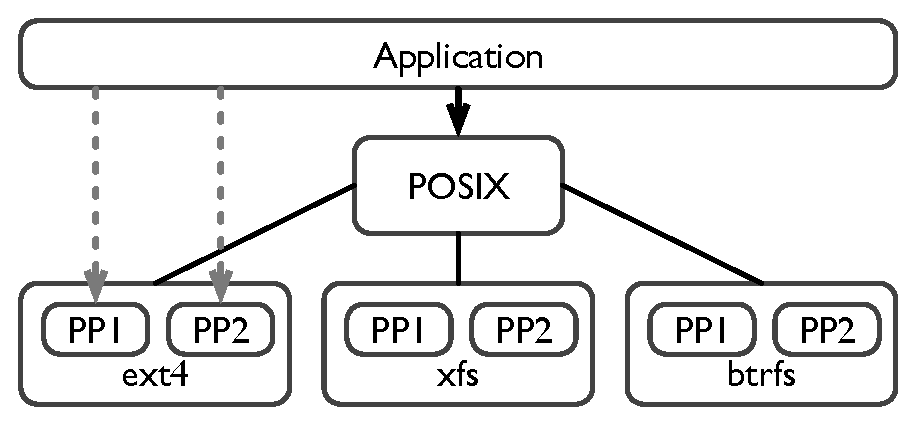
\includegraphics[scale=0.5]{figs/dependencies.eps}
%\vspace{-0.1in}
\mycaption{fig-dependencies}{Application Vulnerabilities}{\footnotesize The
figure shows how an application interacts with different file systems. The
application uses the POSIX standard to interface with file systems. However,
the application also depends on the persistence properties (PP) of ext4. The
grey dotted lines each signify a crash vulnerability in the application. When
the application is run on top of other file systems, the vulnerabilities may
cause application inconsistency in the event of a crash.}
\vspace{-0.2in}
\end{figure}




Since the implementation of system calls vary across file systems, it is hard
to write a correct, efficient update protocol that works across all file
systems. If an update protocol works correctly on one file system, but
incorrectly on another, we say the update protocol has a \textit{crash
vulnerability}: an incorrect assumption about how one or more system calls are
implemented in the underlying file system.  Figure~\ref{fig-dependencies}
illustrates how an application depends upon the persistence properties of ext4:
the application is vulnerable since other file systems may not share these same
properties. 

Crash vulnerabilities are problematic because the underlying assumption (that
certain persistence properties hold) isn't often explicitly mentioned in the
application code. Therefore, when a problem occurs due to an invalid
assumption, it is extremely hard to look at the application code and figure out
the root cause of the problem.  
